%% -- LaTeX packages and custom commands ---------------------------------------
\title{Onlineforecast: An R Package for Adaptive and Recursive Forecasting}

%%tools::toTitleCase("onlineforecast: An R Package for Adaptive and Recursive Forecasting")

\author{by Peder Bacher, Hj\"orleifur G. Bergsteinsson, Linde Frölke, Mikkel L. Sørensen, Julian Lemos-Vinasco, Jon Liisberg, Jan Kloppenborg Møller, Henrik Aalborg Nielsen and Henrik Madsen}

\maketitle

%% - \Abstract{} almost as usual
\abstract{Systems that rely on forecasts to make decisions, e.g.\ control or
  energy trading systems, require frequent updates of the forecasts. Usually,
  the forecasts are updated whenever new observations become available, hence in
  an online setting. We present the \Rprog package \onlineforecast that provides a
  generalized setup of data and models for online forecasting. It has
  functionality for time-adaptive fitting of dynamical and non-linear
  models. The setup is tailored to enable the effective use of forecasts as model
  inputs, e.g.\ numerical weather forecast. Users can create new models for
  their particular applications and run models in an operational setting. The
  package also allows users to easily replace parts of the setup, e.g.\ using
  \del{neural network}\add{new} methods for estimation. The package comes with comprehensive
  vignettes and examples of online forecasting applications in energy systems,
  but can easily be applied for online forecasting in all fields.}






\section[Introduction]{Introduction} \label{sec:intro}

\todo{see
  \url{https://awesomeopensource.com/projects/forecasting}}


Time series analysis and forecasting are indispensable to numerous applied
fields such as business, finance, science and engineering
\citep{cryer2008time}. Time series analysis is the process of statistical
modelling of time series, i.e.\ data which is sampled at different points in
time over a period -- often with a constant increment between the time-points,
i.e.\ equidistant. Classical time series models for a single equidistant time
series use past values of the response variable (model output) as the predictors
(inputs). In this way, appropriate models describing the inherent
auto-correlation structure of the time series can be realized. Examples of these
models include exponential smoothing (e.g.\ Holt-Winters), AutoRegressive (AR),
Moving Average (MA), and the combination of the latter two known as ARMA models. When
multiple correlated time series are available, they can be used as simultaneous model inputs to
improve the forecast. They are then called exogenous variables and the classical
model becomes an ARMAX -- hence the \textit{X} indicates that exogenous input variables
are included. \add{ARMAX models are optimal for forecasting the output of linear
  time invariant (LTI) systems, however for most forecasting applications models
  that can handle non-linear systems are needed. A wide range of techniques for modelling
  non-linear systems exists, either based on input
  transformations or local fitting methods. The \onlineforecast package
  implements an advanced model setup for modelling and forecasting the output of
  non-linear time varying systems. The setup was developed for applications such
  as forecasting wind power \citep{nielsen2002prediction} and thermal loads in
  district heating \citep{nielsen2006modelling}. The significance of the package
  is in the ``online'' term, indicating that at each sampling point the model
  parameter estimates are updated in an effective way for generating multi-step
  forecasts.}

The use of ARMAX models and their variations \add{for forecasting} is still widespread \citep{de200625},
especially \del{in modelling of}\add{for} energy systems due to the high dependency between
variables such as weather, load, renewable generation, and periodic phenomena. Load
forecasting is an obvious example. A nice overview of electric load forecasting
is given by \Citet{Hesham2002} and \citet{hong2016probabilistic}, and for heat
load by \Citet{Dotzauer2002277} who demonstrates the dependency between the
response variable, heat load, and the predictor -- ambient temperature -- using a
piecewise linear function. It is also proposed to model the daily and weekly
diurnal using hours of the week as inputs.


\Citet{BACHER20091772} demonstrated that solar power forecasting
\citep{kleissl2013solar} can be improved by moving from a standard AR model to
an AR model with an exogenous input (ARX), specifically by using numerical
weather predictions (NWPs) as the exogenous inputs. The ARX model uses past
observations and NWPs of global irradiance to forecast the power production from
PV systems and the ARX model obtains higher accuracy than the AR
model. \Citet{bacher2013short} identified exogenous variables that are suitable
for forecasting the heat load of a building, via similar models.

Energy systems are time-varying systems as they usually change over time due to
wear and contamination, like dirt on solar panels or changes in usage. For
example, with new tenants in a house, the dependency between heat load and
other variables, such as calendar time and temperature, changes. Therefore, a forecast
model needs to adapt: the model coefficients are not optimal if they are
constant, they need to be updated and allowed to change over time. The Recursive
Least Square (RLS) method provides a recursive estimation scheme for the
coefficients in regression models, where they are updated at each step, when new
data becomes available. A forgetting factor can be introduced to RLS to
allow for the control of how fast the coefficients can change over time -- this is
referred to as adaptive recursive estimation, with exponential forgetting, in
linear regression and autoregressive models. The method is described by
\Citet{ljung1983theory}, for advances that has been made since then see
e.g.\ \citep{engel2004kernel}.

\add{The objective of the \onlineforecast package is to make it easy to set up and optimize
non-linear \add{models} for generating online multi-step forecasts. The package
contains functionalities not directly available elsewhere, such as:
\begin{itemize}
\item Use of forecasts, e.g.\ NWPs, as input to multi-step forecast models.
\del{\item Application of non-linear models with non-parametric and
  coefficient varying techniques}
\item Optimal tuning of models for multi-step horizons.
\item Recursive estimation for tracking time-varying systems.
\end{itemize}
The package \del{also }provides a framework for handling data and setting up models,
which makes it easy to apply it in a wide range of forecasting applications.}


\subsection{Time series modelling and forecasting in R}

A wide range of existing software for time series forecasting is
currently available \citep{chatfield2019analysis,siebert2021systematic}. Below,
an overview of the currently most relevant \Rprog packages for forecasting is given -- generally, the same functionalities are available in \Python packages.

\del{Exponential smoothing models are popular and simple methods for time series. In
the exponential smoothing past observations are exponentially weighted down,
thus older observations have less impact than newer. The \textit{Holt-Winters}
procedure, where three smoothing constants are used to describe the variation in
time of the parameters, is one of the most famous exponential smoothing
methods. \Citet{doi:10.1287/mnsc.6.3.324} extended the double exponential
smoothing formulation by Holt to capture the seasonality. The
\code{HoltWinters()} function from the
\rpackage{stats}{https://stat.ethz.ch/R-manual/R-devel/library/stats/html/HoltWinters.html}
package estimates parameters of the \textit{Holt-Winters} procedure. The \rpackage{fable}{http://fable.tidyverts.org/} package \citep{fable} provides a
state-space framework to create exponential smoothing models in the function
\code{ETS()}. The function is based on the exponential smoothing framework
presented by \cite{hyndman2008forecasting}. The \rpackage{smooth}{https://cran.r-project.org/package=smooth}
package also provides methods for exponential smoothing.}

Classical ARMAX models can be fitted with the \code{arima()} function from
the \rpackage{stats}{https://stat.ethz.ch/R-manual/R-devel/library/stats/html/00Index.html}
package and the \code{Arima()} function from the
\rpackage{forecast}{https://pkg.robjhyndman.com/forecast/} package
\citep{Hyndman2008} provides automatic model selection with \code{arima()}. \Rprog Packages like
\rpackage{marima}{https://CRAN.R-project.org/package=marima}
\citep{spliid1983fast},
\rpackage{KFAS}{https://cran.r-project.org/package=KFAS},
\rpackage{sysid}{https://cran.r-project.org/package=sysid} and
\rpackage{dlm}{https://cran.r-project.org/package=dlm}
\citep{dlm2010} can also be used for fitting ARMAX models. \Citet{spliid1983fast}
proposed a very fast and simple method for parameter estimation in large
multivariate ARMAX models with a pseudo-regression method that repeats the
regression estimation until it converges. The other packages represent time
series and regression models as state-space models and use a Kalman or Bayesian
filter to include exogenous variables in the model, and optimally reconstruct
and predict the states. \add{Compared to these classical ARMAX models,
  \onlineforecast models offers several advantages, first and foremost the
  recursive fitting scheme which allows for much faster and adaptive fitting. Furthermore, model
coefficients are tuned as a function of the forecast horizon. This optimize the
use of multi-step forecasts as models inputs, such functionality is not available for ARMAX models.}

State-space modelling is frequently used to describe time series data from a
dynamical system, e.g.\ a falling body, see \citep{madsen2007time}. The
dynamical system can in such cases be written as a system of differential
equations or difference equations. State-space models use filter techniques to optimally
reconstruct and predict the states, with examples including the Kalman filter, the extended Kalman
filter, and other Bayesian filters. This gives the possibility of tracking the
coefficients over time, i.e.\ time-varying parameter estimation. The
\rpackage{KFAS}{https://cran.r-project.org/package=KFAS} package
\citep{kfas2017} provides state-space modelling, where the observations come
from the exponential family, e.g.\ Gaussian or Poisson. The
\rpackage{ctsm-r}{http://ctsm.info/} package provides a framework for
identifying and estimating partially observed continuous-discrete time state
space models, referred to as grey-box models. This modelling approach bridges
the gap between physical and statistical modelling using Stochastic Differential
Equations (SDEs) to model the system equations in continuous time and the
measurement equations in discrete time. Packages for discrete time state-space
modelling are:
\rpackage{dlm}{https://cran.r-project.org/package=dlm} for
Bayesian analysis of dynamic linear models,
\rpackage{MARSS}{https://nwfsc-timeseries.github.io/MARSS/} and
\rpackage{SSsimple}{https://cran.r-project.org/package=SSsimple}
for fitting multivariate state-space models. \add{The \onlineforecast models
are basically fitted using a Kalman filter, as explained in Section
\nameref{app:regression}, thus existing packages could be applied. However, the use
of forecasts as model inputs would be very cumbersome and is made very easy with
the onlineforecast setup.}

For non-parametric time series models, the number of available packages is
growing rapidly.\ \rpackage{NTS}{https://cran.r-project.org/package=NTS}
provides simulation, estimation, prediction and identification for non-linear
time series data. It also includes threshold autoregressive models
(e.g.\ self-exciting threshold autoregressive models) and neural network
estimation. \rpackage{tsDyn}{https://cran.r-project.org/package=tsDyn} provides
methods for estimating non-parametric time series models, including neural
network estimation. Neural network, deep learning and machine learning methods
are available in \Rprog\del{ for most methods}. Recurrent neural networks are
available in
the \rpackage{rnn}{http://qua.st/rnn}, the
\rpackage{keras}{https://keras.rstudio.com/} and
\rpackage{tensorflow}{https://github.com/rstudio/tensorflow} packages. Additive
time series models, where non-linear trends are fitted with seasonality
patterns, are available in
\rpackage{prophet}{https://github.com/facebook/prophet}. \add{Time adaptive
  neural networks, i.e.\ with recursive updating, can be implemented in various
  ways \citep{yang2019online}, however currently no effective implementation is available.}

Some packages can be useful for forecast evaluation,
e.g.\ \rpackage{ForecastTB}{https://cran.r-project.org/package=ForecastTB}
presented in \citep{bokde2020forecasttb}. Packages like
\rpackage{forecastML}{https://cran.r-project.org/package=forecastML} and
\rpackage{modeltime}{https://CRAN.R-project.org/package=modeltime} \citep{alexandrov2020gluonts} provide
functionality that simplifies the process of multi-step-ahead forecasting with
machine learning algorithms. The handling of multi-step-ahead
forecasts is also a key feature of the \onlineforecast package. The classical
time series models, such as ARMAX and Exponential Smoothing models, are mostly
optimal for modelling Linear Time Invariant (LTI) systems, however, most systems
are not LTI. Furthermore, since a model is always a simplification of reality,
optimal multi-step forecasting is often not possible with the classical models,
especially when using exogenous inputs. For optimal multi-step ahead forecasting
the models must be tuned for each horizon -- which is exactly what the
\onlineforecast package does.

\subsection{\del{Implementation}\add{Functionality} of onlineforecast}

\del{The \onlineforecast package builds on an advanced model setup for
forecasting. This model setup was developed for applications such as forecasting
wind power \citep{nielsen2002prediction} and thermal loads in district heating
\citep{nielsen2006modelling}. The significance of the package is in the
``online'' term, indicating that the model is updated when new observation
becomes available -- recursively updating the coefficients and generating new
forecasts at every point in time.}

\del{The objective of the package is to make it easy to set up and optimize models
for generating online multi-step forecasts. The package contains functionalities
not directly available elsewhere:
\begin{itemize}
\item Use of forecasts, e.g.\ NWPs, as input to multi-step forecast models.
\item Application of non-linear models with non-parametric and
  coefficient varying techniques.
\item Optimal tuning of models for multi-step horizons.
\item Recursive estimation for tracking time-varying systems.
\end{itemize}
The package also provides a framework for handling data and setting up models,
which makes it easy to apply in a wide range of forecasting applications.}


A model is an approximation to the real world, thus it will always be a
simplification and can never predict real-world data. One of the main challenges of
identifying a good forecast model is to find the most informative input
variables and the best structure of the model. The \onlineforecast package
provides functionality for defining, validating and selecting models in a
systematic way.

To introduce the \onlineforecast models consider the simplest model with one
input. It is the linear model for the $k$'th horizon
\begin{align}
    Y_{t+k|t} = \beta_{0,k} + \beta_{1,k} u_{t+k|t} + \varepsilon_{t+k|t}
\end{align}
where $Y_{t+k|t}$ is the response variable and $u_{t+k|t}$ is the input
variable. The coefficients are $\beta_{0,k}$ and $\beta_{1,k}$, note that they
are subscripted with $k$ to indicate that they are estimated for
\add{individually for every}\del{each} horizon. The error $\varepsilon_{t+k|t}$
represents the difference between the model prediction and the observed value
for the $k$-step horizon. The interpretation of the subscript notation $t+k|t$
on a variable is, that it is the $k$-step prediction calculated using only
available information at time $t$, usually referred to either ``conditional on
time $t$'' or ``given time $t$''.

The options for estimating the coefficients in the package are either the Least Squares
(LS) or Recursive Least Squares (RLS) method. In the LS method, the coefficients
are constant, while the in RLS method the coefficients can change over time
\begin{align}
    Y_{t+k|t} = \beta_{0,k,t} + \beta_{1,k,t} u_{t+k|t} + \varepsilon_{t+k|t}
\end{align}
as indicated by the subscript $t$ on the coefficients. This allows for tracking
changes occurring over time.

The package allows for easy definition of transformations and thus the
  possibility to fit non-linear models e.g.
\begin{align}
    Y_{t+k|t} = \beta_{0,k,t} + \beta_{1,k,t} f(u_{t+k|t};\alpha) + \varepsilon_{t+k|t}
\end{align}
where the function $f(u_{t+k|t};\alpha)$ is some non-linear function of the
input $u_{t+k|t}$ with parameter $\alpha$, e.g.\ a low pass filter on the outdoor
temperature to model building heat dynamics. The package sets up tuning of the
non-linear function parameters, e.g.\ if the parameter $\alpha$ determines the
degree of low-pass filtering it can be tuned with an optimizer to match the
dynamics of the system at hand.

An example of generated forecasts can be appreciated in Figure
\ref{fig:forecastsExample}. Hourly forecasts up to 36 steps ahead of heat load
in a single building are shown for three consecutive steps. This is the typical
structure of forecasts generated with the package. It can be seen how
the forecasts change slightly as they are updated in each step, e.g. around
12:00 \del{at day 2}\add{the second day}, hence horizon $k=23$ in the upper plot, which corresponds to $k=21$ in the lower plot.
\begin{figure}
\centering
\begin{knitrout}
\definecolor{shadecolor}{rgb}{0.969, 0.969, 0.969}\color{fgcolor}
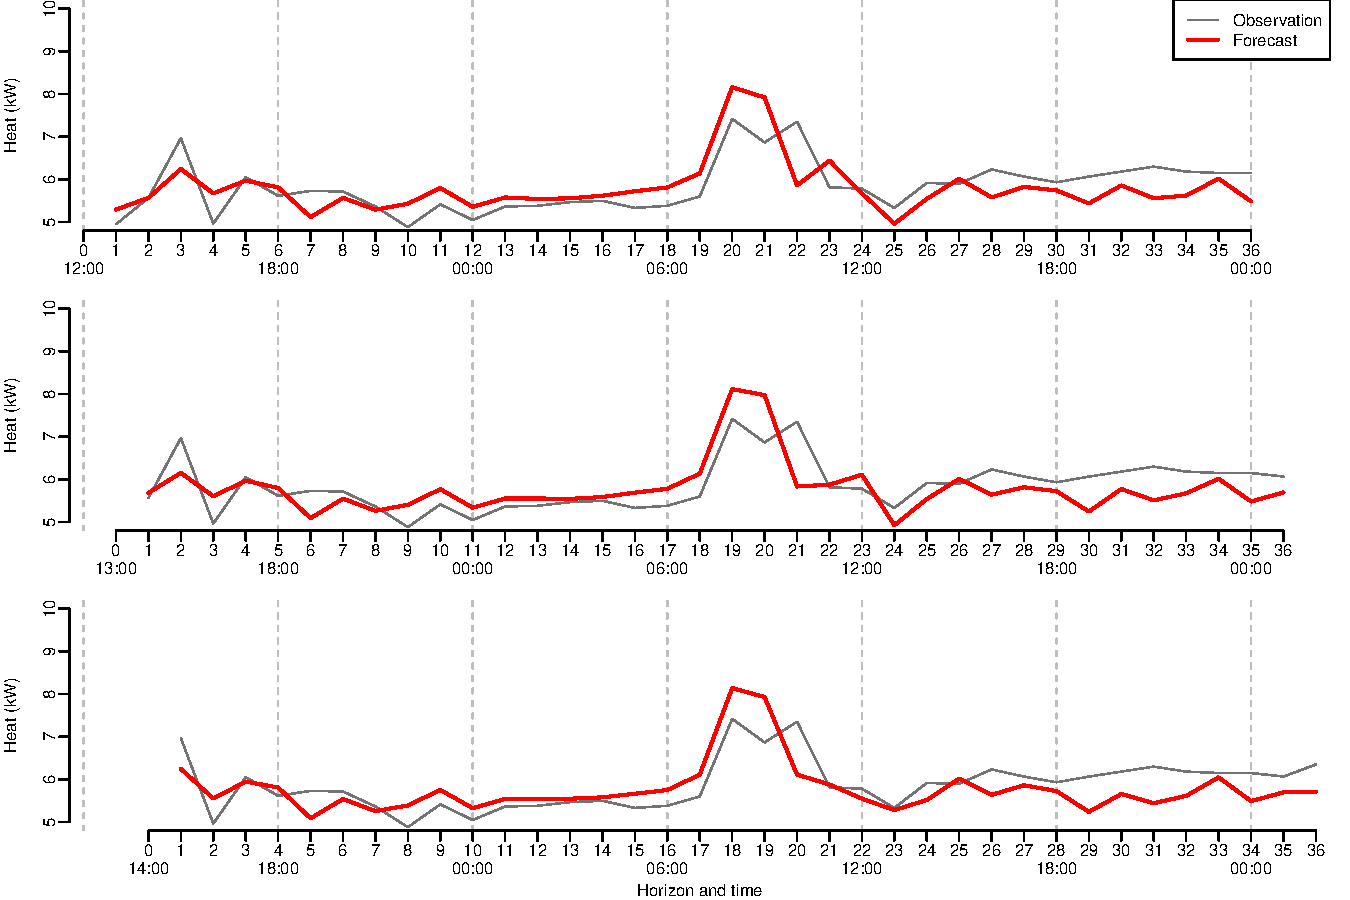
\includegraphics[width=1\linewidth]{tmp/genfig/unnamed-chunk-8-1} 
\end{knitrout}
\caption{Example of hourly load forecasts at three
  consecutive time steps. The upper is calculated at 12:00, the middle is
calculated at 13:00 and the lower at 14:00. It can be seen how the forecasts change
slightly as they are updated in each step, most clearly seen around 12:00 on \del{day
2}\add{the second day}.}\label{fig:forecastsExample}
\end{figure}

\FloatBarrier

\subsection{Vignettes}\label{subsec:vignettes}
A great way to get hands-on experience with the package is through vignettes. They are
available when installing the package and on the website
\href{https://onlineforecasting.org}{onlineforecasting.org}, where also examples
of different forecast applications can be found. The package vignettes are:
\begin{itemize}
\item \vignette{setup-data} covers how data must be set up. The
  vignette goes into detail on how observations and model inputs
  (forecasts) are set up. The vignette also focuses on the importance of
  aligning forecasts correctly in time.
\item \vignette{setup-and-use-model} focus on how to set up a model and use it
  to generate forecasts.
\item \vignette{model-selection} demonstrates how model selection
  can be carried out.
\item \vignette{forecast-evaluation} covers the evaluation of forecasts, and how to
  use this information to improve a model.
\item \vignette{online-updating} demonstrates how to update an operational model when new observations become available. This functionality is not
  covered in the \Rprog examples in the present paper.
\end{itemize}

Furthermore, one vignette is available only on the website:
\begin{itemize}
\item \vignette{nice-tricks} provides some useful tips on how to
  make the workflow easier with the package.
\end{itemize}


\subsection{Paper structure}

The paper is structured as follows: In Section
\nameref{sec:model-forecast-matrix} the notation used in the paper and how to set up
data is introduced. The core methodology is presented in Section
\nameref{sec:two-stage-modelling} and important aspects of forecast modelling are
outlined in Section \nameref{sec:model-select-valid}. In Section
\nameref{sec:example-with-r-code} examples with \Rprog code are presented to provide a
short hands-on tutorial. The paper ends with a summary and conclusions in Section
\nameref{sec:summary}.

In addition, three appendices are included with the paper. In Appendix
\nameref{sec:forec-model-notat} some guidelines on the mathematical notation of
forecast models are provided. In \del{Appendix \nameref{app:transformation-of-inputs}
the functions used for transformations are detailed and in }Appendix
\nameref{app:regression} the regression schemes are covered in full detail.


\section{Notation and forecast matrices}\label{sec:model-forecast-matrix}
The notation in this article follows \cite{madsen2007time} as close as possible. All time series considered are equidistantly sampled and the sampling period is normalized to 1. Hence, the time $t$ is simply an integer indexing the value of a variable at time $t$. The same goes for $k$ which indexes the forecast horizon $k$ steps ahead. In the \onlineforecast setup, forecasts are calculated at time $t$ for each
horizon up to $\nk$ steps ahead. To achieve the desired notation that can
deal with overlapping time series, a two dimensional index is required. The
notation used is
\begin{align}
  u_{t+k|t}
\end{align}
which translates to: the value of variable $u$ at time $t+k$ \emph{conditional}
on the information available at time $t$. The conditional term is indicated
by the bar $|$. Thus, for $k > 0$ this is a forecast available at $t$ and $k$ is
the horizon. When writing a forecast model the following convention is used
\begin{align}
  Y_{t+k|t} = \beta_{0,k} + \beta_{1,k} u_{t+k|t} + \varepsilon_{t+k|t}
\end{align}
where $Y_{t+k|t}$ is the model output, $\beta_{0,k}$ and $\beta_{1,k}$ are the
coefficients and $\varepsilon_{t+k|t}$ with
$\mathrm{Var}(\varepsilon_{t+k|t})=\sigma^2_k$ is the error. The error process
and variance $\sigma^2_k$ is thus separate for each horizon. Note, that the
model is fitted separately for each horizon, so the coefficients take different
values for each horizon, and the predictions and errors are separated for each
horizon. This was a simplified example, see Appendix \nameref{sec:forec-model-notat}
on how to write the full forecast models.


\subsection{Forecast matrix}

A forecast matrix is the format of forecast data in the onlineforecast setup. 
See examples in the \vignette{setup-data} vignette. Data
must have this format in order to be used as model input, and the forecasts
are generated in this format. The forecast matrix holds for any time past
\emph{the latest available forecast along the row} for the corresponding time
\begingroup
% padding
\setlength\arraycolsep{5pt} % space between columns
\renewcommand*{\arraystretch}{2} % space between rows
\begin{align}\label{eq:minput-def}
  \mB{u}_n = 
  \begin{blockarray}{cccccc}
    %%
    \textbf{k0} & \textbf{k1} & \textbf{k2} & \ldots & \textbf{k$n_k$} & \rightarrow\textbf{horizon/time}\downarrow\\
    \begin{block}{(ccccc)c}
      %%
      u_{1|1} & u_{2|1} & u_{3|1} & \ldots &
      u_{1+\nk|1} & 1\\    
      u_{2|2} & u_{3|2} & u_{4|2} & \ldots &
      u_{2+\nk|2} & 2\\    
      \vdots & \vdots & \vdots &  & \vdots & \vdots\\
      %%
      u_{t-1|t-1} & u_{t|t-1} & u_{t+1|t-1} &
      \ldots & u_{t-1+\nk|t-1} & t-1\\
      %%
      u_{t|t} & u_{t+1|t} & u_{t+2|t}  &
      \ldots & u_{t+\nk|t} & t\\
      \vdots & \vdots & \vdots &  & \vdots & \vdots\\
      u_{n|n} & u_{n+1|n} & u_{n+2|n}  &
      \ldots & u_{n+\nk|n} & n\\
      %%
    \end{block}
  \end{blockarray}
\end{align}
\endgroup
where 
\begin{itemize}
\item $t$ is the counter of time for equidistant time points with
  sampling period of 1 (note that $t$ is not included in the matrix, it
  is simply the row number).
\item $n$ is the number of time points in the matrix. Hence, the data is
  available and can be used as model input at time $t=n$.
\item \nk is the longest forecasting horizon.
\item The column names (in \Rprog) are indicated above the matrix, they are simply
  a '{\bf k}' concatenated with the value of $k$, e.g.\ $n_k$ in the last column.
\end{itemize}

Note, that the $\textbf{k0}$ column holds values with forecast horizon $k=0$,
which could be real time observations. Usually, only the horizons to be
forecasted should be included, hence often $\textbf{k0}$ is not needed. For example with a prediction horizon $\nk=24$ at $t = 100$, we will have the
forecast matrix
\begingroup
% padding
\setlength\arraycolsep{5pt} % space between columns
\renewcommand*{\arraystretch}{2} % space between rows
\begin{align}
\mB{u}_{100} = 
\begin{blockarray}{cccccc}
  %%
  \textbf{k0} & \textbf{k1} & \textbf{k2} & \dots & \textbf{k24} & \rightarrow\textbf{horizon/time}\downarrow\\
  \begin{block}{(ccccc)c}
      u_{1|1} & u_{2|1} & u_{3|1} &
      \ldots & u_{25|1} & 1\\
      %%
      u_{2|2} & u_{3|2} & u_{4|2} &
      \ldots & u_{26|2} & 2\\
      %%
      \vdots & \vdots &  \vdots &  & \vdots & \vdots \\
      %%
      u_{99|99} & u_{100|99} & u_{101|99} &
      \ldots & u_{123|99} & 99\\
      %%
      u_{100|100} & u_{101|100} &
      u_{102|100}  & \ldots & u_{124|100} & 100\\
  \end{block}
\end{blockarray}
\end{align}
\endgroup
In Section \nameref{sec:setup-of-data} examples of how data and forecast matrices are set up in \Rprog are given.


\section{Two-stage modelling procedure} \label{sec:two-stage-modelling}

Two-stage modelling procedure is a widespread approach to modelling non-linear
functional relations between inputs and outputs (see e.g.\ \cite{breiman1985estimating} and \cite{weisberg2005applied} for direct
transformation of predictor variables, and \cite{hastie2009elements} for
non-parametric transformation techniques). Using
transformations allows for fitting complex models with robust and fast
estimation techniques. In the first stage, the \emph{transformation stage}, the
inputs are mapped by some function -- potentially into a higher dimensional
space. In the second stage, the \emph{regression stage}, a linear regression
model\footnote{In the remaining of the text, when the term ``regression'' is
used it is implicit that it is ``linear regression''.} is applied between the
transformed inputs and the output.

As an example, a model with two inputs is presented. In this model the
transformation stage consists of generating an intercept and mapping the two
inputs (they are set up as forecast matrices $\mB{u}_{1,t}$ and $\mB{u}_{2,t}$)
\begin{align}\label{eq:transformation-stage-example}
  \text{Intercept:}&\quad x_{0,t+k|t} = 1 \\[1ex]
  \text{Input 1:}&\quad x_{1,t+k|t} = f_1(u_{1,t+k|t}, \mB{\alpha}\n{1})\\[1ex]
  \text{Input 2:}&\quad \mB{x}_{2,t+k|t} = f_2(u_{2,t+k|t}, \mB{\alpha}\n{2})
\end{align}
where the $f$'s are transformation functions that map the inputs to
regressors. Note, that the intercept is simply a constant passed on to the
regression. The transformations result in multiple inputs for the regression --
the latter actually as multiple variables indicated by the bold font
notation. In the regression stage the linear model
\begin{align}\label{eq:regression-stage-example}
  Y_{t+k|t} = \beta_{0,k} x_{0,t+k|t} + \beta_{1,k}
  x_{1,t+k|t} + \mB{\beta}^T_{2,k} \mB{x}_{2,t+k|t} + \varepsilon_{t+k|t}
\end{align}
is fitted. The regression is carried out separately for each horizon $k$. Thus, the combined model has:
\begin{itemize}
\item An intercept
\item Two inputs: $u_{1,t+k|t}$ and $u_{2,t+k|t}$
\item Output: $Y_{t+k|t}$
\item Transformation functions: $f_1$ and $f_2$
\item Transformation parameters: $\mB{\alpha}\n{1}$ and $\mB{\alpha}\n{2}$
\item Regression coefficients: $\beta_{0,k}$, $\beta_{1,k}$ and
  $\mB{\beta}_{2,k}$
\end{itemize}

Some transformation parameters should be optimized for the data at hand, e.g.\ a
low-pass filter coefficient depends on the system dynamics. The same goes for
some parameters related to the regression scheme, e.g.\ the forgetting factor
(introduced below). We will refer to them together as {\bf\emph{offline parameters}}.
The \onlineforecast package provides a setup, where the offline parameters
can be optimized using a heuristic optimization (e.g.\ a BFGS quasi-Newton
method). The default score, which is minimized, is the Root Mean Square Error
(RMSE) of the predictions -- hence offline parameters in the
model above, given data from the period, $t = 1,2,\dots,n$, are \del{found}\add{optimized} by
solving
\begin{align}\label{eq:rmse-score}
  \min_{\mB{\alpha}\n{1}, \mB{\alpha}\n{2}} \quad & \frac{1}{n-k}\sum_{t=1}^{n-k} (y_{t+k} -
  \hat{y}_{t+k|t}(\mB{\alpha}\n{1}, \mB{\alpha}\n{2}))^2
\end{align}
Naturally, other scores can be minimized (e.g.\ MAE or the Huber psi-function,
however the regression schemes should be modified accordingly, which is not
trivial).

The regression coefficients are calculated with a closed-form scheme: either
with the Least-Squares (LS) or the Recursive Least-Squares (RLS) scheme -- in
the latter the coefficients are allowed to vary over time. In both schemes the
coefficients \add{are gathered in the vector
$\mB{\beta}_{k}$ and} calculated separately for each horizon
$k$. In Appendix \nameref{app:regression} both schemes are presented in full detail.

In the LS scheme the coefficients \del{are gathered in the vector
$\hat{\mB{\beta}}_{k}$, which is}\add{are} constant \del{in}\add{during} the entire period. The output
vector is $\mB{y}_{k,n}$ and for a given value of the transformation parameters
(i.e.\ here $\mB{\alpha}\n{1}$ and $\mB{\alpha}\n{2}$) the transformed data is
calculated and set up in the design matrix $\mB{X}_{k,n}$. The LS coefficients
are then calculated by
\begin{align}
  \hat{\mB{\beta}}_{k} = (\mB{X}_{k,n}\mB{X}_{k,n})^{-1} \mB{X}_{k,n}\mB{y}_{k,n}
\end{align}
and the predictions calculated by
\begin{align}
  \hat{\mB{y}}_{k,n} = \mB{X}_{k,n} \hat{\mB{\beta}}_{k}
\end{align}
where $\hat{\mB{y}}_{k,n} = \left[ \hat{y}_{1+k|1} ~~
    \hat{y}_{2+k|2} ~~ \dots ~~ \hat{y}_{n|n-k}\right]^T$ are the
predictions. Note, that for the LS scheme the predictions are ``in-sample'',
since \add{data} from the entire period is used for the coefficient calculation.

In the RLS scheme the coefficients are calculated recursively, meaning that they
are updated \del{at each time $t$ when stepping through the period}\add{in every
time step -- the RLS is actually a Kalman filter with the model coefficients
in the state vector. At each time $t$ the coefficients are updated by
\begin{align}
  \mB{R}_{k,t} &= \lambda \mB{R}_{k,t-1} + \mB{x}_{k,t} \mB{x}^T_{k,t}\\
  \hat{\mB{\beta}}_{k,t} &= \hat{\mB{\beta}}_{k,t-1} + \mB{R}^{-1}_{k,t}
  \mB{x}_{k,t} (y_t - \mB{x}^T_{k,t} \hat{\mB{\beta}}_{k,t-1})
\end{align}
and the predictions by
\begin{align}
  \hat{y}_{t+k|t} = \mB{x}_{t+k|t} \hat{\mB{\beta}}_{k,t}
\end{align}
where $\mB{x}_{k,t}$ is the data available for horizon $k$ at time $t$ (a row in
the design matrix $\mB{X}_{k,n}$), and $\mB{x}_{t+k|t}$ is the $k$'th horizon
transformed input forecast available at time $t$, see the appendix for
all details. }\del{In each update only the
``newly'' obtained data at $t$ is used, thus only past data goes into the calculations, which makes the
calculated RLS coefficients and predictions ``out-of-sample'' (opposed to
LS). Furthermore, The updating scheme allows the coefficients to vary such that
the model adapts to data over time. When writing the model as in Equation
\eqref{eq:regression-stage-example} this can be indicated with a $t$ subscript
on the coefficients, i.e.\ $\beta_{0,k,t}$, $\beta_{1,k,t}$ and
$\mB{\beta}_{2,k,t}$. }The \add{coefficients adapts to data over time and the }level of adaptivity \del{can be}\add{is} controlled by the
forgetting factor $\lambda$ \del{in the RLS scheme } (with value between 0 and 1). When
$\lambda=1$, all past data at $t$ is equally weighted. When $\lambda < 1$, higher
weight is put on recent data -- the smaller the value, the faster the model
adapts to \add{recent} data. By optimizing the forgetting factor as an offline
parameter, the model adaptivity can be tuned\del{ to optimally track system changes over time}.


An important point to notice is that the offline parameters are always constant
for the given period, hence all predictions are essentially
``in-sample''. However, depending on the regression scheme there is a
difference: with the LS scheme the regression coefficients \add{are calculated once using all data}\del{are constant through
the period}, thus the predictions are (fully) ``in-sample'', where as with the
RLS scheme they adapt through the period and the predictions are
``out-of-sample'' (\del{i.e.\ }except for the offline parameters). This makes a
difference, since model overfitting is less of a problem when using the RLS
scheme\del{, although still problems can occur, e.g.\ if the forgetting factor is
\del{optimized to be }close to 1, because no systematic change occurred in the
training period, but changes appear in new data}.

The typical \onlineforecast setup is to optimize the (usually few) offline
parameters in an ``offline'' setting, but calculate the regression coefficients
adaptively with the RLS. This has the advantage that the model adapts and tracks
the systematic changes in input-output relations, while keeping the setup
computationally very effective -- updating the coefficients and calculating a
forecast at each time $t$ takes few operations\del{, since only the newly
  available data is used}. The\del{ more computationally heavy} optimization of
offline parameters can be carried out when computational resources are available
(e.g.\ every week for hourly forecasts).

\del{In the following sections more information, on the package functions
for the two stages, are presented.}


\subsection{Transformations\del{ stage}}\label{sec:transf-stage}

In the transformation stage the inputs are mapped using some function as
demonstrated above, for more examples, see the \vignette{setup-and-use-model}
vignette. The \onlineforecast package has functions available for most common
use, however it is easy to write and use new functions as they are simply \Rprog
functions. \add{The main functionality they have to fulfil is to}\del{which}
return a forecast matrix (or a list of them)\add{, which is also the reason why
some of the regular \Rprog functions and operators has been extended for the
multi-horizon setup, e.g.\ for splines as explained below}. For \add{\Rprog}
examples, see Section \nameref{sec:defining-model}\add{ and the
  vignettes}. The currently available transformation functions are:

\begin{itemize}
\item Low-pass filtering, \code{lp()}: A low-pass filtering for modelling
  linear dynamics as a simple RC-model. See e.g.\ \cite{nielsen2006modelling}
  for further information.
\item Basis splines, \code{bspline()}: Use the \code{bs} function for
  calculating regression splines basis functions.
\item Periodic basis splines, \code{pbspline()}: Use the \code{pbs} function
  for calculating periodic regression splines basis functions.
\item Fourier series, \code{fs()}: Fourier series as periodic regression basis
  functions.
\item Auto-regressive, \code{AR()}: For including Auto-Regressive (AR) terms.
\item Intercept, \code{one()}: Generates a forecast matrix of ones,
  i.e.\ intercept.
\end{itemize}

In the following section, the low-pass filtering is shortly described
below. \add{For more examples of transformations, see the package vignettes.}\del{
In Appendix \nameref{app:transformation-of-inputs} the other transformation
function are presented and in Section \nameref{sec:example-with-r-code} a full
example with \Rprog code is provided.}

The implementation in \onlineforecast allows all parameters which are used in
some way (except the regression coefficients) to be included in an optimization,
using any available optimizer i \Rprog. This includes e.g.\ the RLS forgetting
factor, knot points or order of splines, i.e.\ both continuous and integer
variables. This functionality is achieved using a simple syntax as explained in
Section \nameref{sec:example-with-r-code}.


\subsubsection{\it Low-pass filtering}
%{\it Low-pass filtering}
\label{sec:low-pass-filtering}

When modelling time series from linear dynamical systems, the classical ARMAX
model is often the optimal choice \citep{madsen2007time}. However, for
multi-step forecasting, this is often not the case, especially for longer
horizons. In the \onlineforecast setup, where the regression model is fitted for
each horizon, a ``trick'' can be used for modelling linear dynamics: simply
apply a filter on the input and then use the filtered input in the regression
stage. For example, dynamics between ambient air temperature and \del{indoor temperature}\add{heat demand} are slow due to the thermal mass of the
building.\del{Therefore, it is reasonable that the dynamics between
the ambient air temperature and the heat demand (when keeping a desired indoor
temperature)}\add{ Thus they} can
be modelled using a low-pass filter\del{. This technique is successfully applied for
energy modelling using physical knowledge}, see \cite{nielsen2006modelling} for
modelling heat load in district heating and \cite{bacher2013short} for
forecasting single buildings heat load.

In the package the simple low-pass filter
\begin{align}
  x_{t+k|t} = \frac{(1-a) u_{t+k|t}}{1-a x_{t-1+k|t-1}}
\end{align}
is implemented. The filter coefficient $a$ must take a value between 0 and 1 and
should be tuned to match the time constant optimal for the particular
data. When the current implemented low-pass filter is applied in the
transformation stage on some forecast matrix $\mB{u}_{t+k|t}$, the filter is
applied on each column, i.e.\ independently for each horizon $k$. More advanced
filters can also be implemented.\del{ See Appendix
\nameref{sec:low-pass-filtering-appendix} for a more detailed description.}

\del{
\subsection{Regression stage}}

\del{
As described above and in full detail in Appendix \nameref{app:regression}, the
regression model takes transformed data from a period $t = 1,2,\dots,n$ and is
fitted separately for each horizon $k$, i.e.\ the model structure remains the
same, only the coefficients change with the horizon.\del{ In the presented example, the regression model is as stated in Equation
\eqref{eq:regression-stage-example} -- it is implicit that the regression is
linear and that the coefficients are calculated using the}. The two
  implemented schemes, LS and RLS, are both closed-form minimization of the
$\mathit{RMSE}$ of the predictions. The main differences between the two schemes
have been outlined above and it should be clear that in most settings the RLS is
preferable.}

\del{
Two fundamental assumptions are behind the optimality of least squares
predictions\del{, hence the minimizing the $\mathit{RMSE}$}. Both assumptions are
related to error process $\varepsilon_{t+k|t}$ in such models:
\begin{itemize}
  \item The one-step error $\varepsilon_{t+1|t}$ is white noise, hence a
    sequence of independent, identically distributed (i.i.d.) random variables,
  \item They are drawn from a normal distribution, i.e.\ $\varepsilon_{t+k|t}
    \sim N(0,\sigma^2_k)$.
\end{itemize}
The latter assumption is not very important, since first of all the least
squares ensures the best and un-biased estimation of the conditional mean, which
is often the wanted and optimal point prediction \citep{madsen2007time}. For
example, one important feature is that sums of least squares predictions are
also un-biased, e.g.\ the daily sum of hourly LS predictions are good
predictions of the daily total. The i.i.d.\ assumption should be checked during
model validation, as described in the following section.\del{, with the
Auto-Correlation Function (ACF) for the one-step ahead residuals, as well as the
Cross-Correlation Function (CCF) between the one-step ahead residuals and the
inputs, as demonstrated by \cite{bacher2013short}}.}


%% \subsubsection{Recursive least squares}

%% The $k$ step prediction at time $t$ is
%% \begin{align}
%%   \yhat{}{t+k|t} = \hat{\beta}_{0,k} + \hat{\beta}_{1,k} x_{t+k|t}
%% \end{align}
%% Note, that the hat is reserved for predictions and estimates
%% calculated using the statistical model, thus the hat is not on the
%% inputs, which are however often predictions (NWPs). If models are fitted in
%% several stages, e.g.\ the inputs in the final model are actually first
%% predicted using another model, then the hat is removed on the inputs
%% in the final model.

%% In the above model there are in total $t \cdot \nk$ output ($Y$) random
%% variables, as well as there are $t \cdot \nk$ error random variables.


%% ??This model is easily setup by selecting the corresponding column for
%% $k$ of the ?? input matrix, see??.




\section{Model selection and validation} \label{sec:model-select-valid}

\subsection{Model selection}

In statistics, different model selection procedures are used
\citep{madsen2010introduction}. Essentially, a backward or a forward selection
procedure can be applied, or some combined approach. In the \onlineforecast
package both procedures are implemented, as well as a combined
approach\del{. The following is a short description of the stepping process of
  each procedure implemented, for examples of this} (see the
  \vignette{model-selection} vignette for examples).

In each step of the selection process two properties of the model can be modified:
\begin{itemize}
\item Model inputs: In each step, inputs can either be removed or added.
\item Integer offline parameters: In each step integer parameters, such
  as the number of knot points in a basis spline or the number of harmonics in a
  Fourier series can be incremented or decremented.
\end{itemize}

In each step of the process, the offline parameters are first optimized to
minimize the score for each modified model (in most cases the appropriate score
is the RMSE in Equation \eqref{eq:rmse-score} summed for selected horizons). Then the scores of the modified
models are compared with the score of the currently selected model and the model
with the lowest score is selected for the next step. This continues until no
further improvement of the score is achieved and the model with the lowest score is
selected. It is important to note, that the implemented procedure should only
be used with the RLS scheme, with the LS scheme the score is calculated fully
in-sample leading to overfitting.\del{ For the LS an $F$-test should be applied
however that is currently not implemented.}

\del{A model must be given to initialize the stepping process. A backward selection
will start with the full model and one-by-one remove inputs and count down
parameters. A forward selection will start with the null model and, taking from
a provided full model, add inputs and count up parameters.  If the direction
``both'' is set then in each step, inputs will either be removed or added, and
parameters will be counted both up and down.}


\subsection{Model validation}

The most important aspects of validation of forecast models are discussed in
this section (see the \vignette{forecast-evaluation} vignette for examples).

\subsubsection{\it Training and test set}

One fundamental problem in data-driven modelling is overfitting. This
can easily happen when the model is fitted (trained) and evaluated on the same
data. There are essentially two ways of dealing with this: penalize increased
model complexity (regularization) or divide the data into a training set and
test set (cross-validation) \citep{tashman2000out}. In most forecasting applications the easiest and most transparent approach is
cross-validation -- many methods for dividing into sets are possible. In
the \onlineforecast setup, when a model is fitted \add{recursively }using\del{a recursive
  estimation method (like} the RLS, only past data is used when calculating the regression
coefficients, so there is \del{no}\add{little} need for dividing into a training and a test
set.

The offline parameters (like the forgetting factor and low-pass filter
coefficients) are optimized on a particular period, hence overfitting is
possible, however, typically, only very few parameters compared with the number
of observations are estimated -- so it is very unlikely that a
recursively-fitted model will overfit.\del{ For non-recursive fitting, it is naturally important to divide into a training
and a test set -- which is easily done in the \onlineforecast setup using the
\code{scoreperiod} variable as demonstrated in Section
\nameref{sec:example-with-r-code}.}


\subsubsection{\it Scoring}
The scoring of forecasts can be done in many ways, however in the
\onlineforecast package,
where the conditional mean is estimated and when using the RLS scheme,
we recommend choosing the Root Mean Square Error (RMSE) in Equation
\eqref{eq:rmse-score} as the best score to use. When using the LS scheme it can
be favourable to include regularization penalty  to avoid overfitting, hence AIC or BIC
is preferable. One important point when comparing forecasts is to only include the complete
cases, i.e.\ forecasts at time points with no missing values across all horizons
and across all evaluated models. A function for easy selection of only complete
cases given multiple forecasts is implemented, see the examples in Section
\nameref{subsec:evaluation}.


\subsubsection{\it Residual analysis}
Analysing the residuals is an important way of validating that a model cannot be
further improved or learning how it can improved. The main difference from
classical time series model validation, where only the one-step ahead error is
examined, is that multiple horizons should be included in the analysis. The two
most important ways of analyzing the residuals are to:
\begin{itemize}
\item Plot residual time series to find where large forecast errors occur.\del{ The
  accumulated residuals are also often useful to examine, e.g.\ cumulative
  squared error plot.}
\item Plot scatter plots of the residuals vs. other variables to see if there
  are any apparent dependencies not captured by the model.
\end{itemize}

In order to dig a bit more into the result of \del{the}\add{a} recursive
estimation, the regression coefficients can be plotted over time. In this way,
it is possible to learn how the relations between the variables in the model
evolve over time. If large changes are found in some periods it might be
worthwhile to zoom into those periods to learn what causes these \add{changes}
and how to potentially improve the model. In case auto-correlation is left in
the residuals, an error model can be used to improve the forecasts by applying
an auto-regressive model on the residuals. This is somewhat equivalent to
include an MA part in the original model\del{ (which is not implemented as it is
  far from trivial)}.

As summarizing measures for validation of how well dynamics are modelled:
\begin{itemize}
\item Plot the auto-correlation function (ACF) of the one-step residuals.
\item Plot cross-correlation functions from one-step residuals to other
  variables, see \citep{bacher2013short}.
\end{itemize}
Systematic patterns found in these functions lead to direct knowledge on how to
improve the model, see for example the table on page 155 in
\cite{madsen2007time}\del{ and the examples in Section \nameref{subsec:evaluation}
  in the present paper}.


\section{Example with R code} \label{sec:example-with-r-code}

A short introduction to the functionalities and steps in setting up a
model is given in the following -- for more details\del{ and functionalities}, see the
vignettes listed in Section \nameref{subsec:vignettes} and the website \href{https://onlineforecasting.org}{onlineforecasting.org}.


First, a few remarks on the implementation. \onlineforecast models are set up
using an object-oriented R6 class. The main reason for this is that \code{R6}
objects use reference pointers, which allows to make minimum changes in
computer memory when updating a model fit with new data -- this would not be
possible with the regular S3 class objects, as they are always copied in memory
when updated by a function.

Furthermore, it is noted, that model inputs and transformations simply are
defined using \Rprog code. The regular \code{formula} class is not used, since
it cannot operate as needed on the multi-horizon forecast matrices. The provided
code for the inputs defines the transformations etc.\ and is executed for each
input to generate the data used for regression.


\subsection{Setup of data} \label{sec:setup-of-data}



\noindent Data must be set as variables in a list, here we have
loaded \code{D} with the data for the examples:
\begin{knitrout}
\definecolor{shadecolor}{rgb}{0.969, 0.969, 0.969}\color{fgcolor}\begin{kframe}
\begin{alltt}
\hlkwd{class}\hlstd{(D)}
\end{alltt}
\begin{verbatim}
## [1] "data.list" "list"
\end{verbatim}
\end{kframe}
\end{knitrout}
As seen its class is \code{data.list}, which is inherited from the
\code{list} class. Hence, it is simply a \code{list} extended with some modified
and new functions (can be listed with \code{methods(class="data.list")}).

All inputs to be used must be formatted as forecast matrices and set in the list
as \code{data.frame}s. For example the ambient temperature forecasts:
\begin{knitrout}
\definecolor{shadecolor}{rgb}{0.969, 0.969, 0.969}\color{fgcolor}\begin{kframe}
\begin{alltt}
\hlkwd{class}\hlstd{(D}\hlopt{\$}\hlstd{Ta)}
\end{alltt}
\begin{verbatim}
## [1] "data.frame"
\end{verbatim}
\begin{alltt}
\hlkwd{head}\hlstd{(D}\hlopt{\$}\hlstd{Ta[ ,}\hlnum{1}\hlopt{:}\hlnum{8}\hlstd{],} \hlnum{4}\hlstd{)}
\end{alltt}
\begin{verbatim}
##         k1       k2      k3      k4       k5       k6       k7       k8
## 1 -2.82340 -3.20275 -3.1185 -3.0896 -3.13200 -3.16130 -3.16645 -3.08885
## 2 -2.90405 -3.11850 -3.0896 -3.1320 -3.16130 -3.16645 -3.08885 -2.77165
## 3 -2.93590 -3.08960 -3.1320 -3.1613 -3.16645 -3.08885 -2.77165 -2.32185
## 4 -2.89315 -3.11285 -3.0484 -3.1090 -3.11600 -2.80990 -2.36895 -2.00945
\end{verbatim}
\end{kframe}
\end{knitrout}
\noindent The time must be in a \code{POSIXct} vector named \code{t}:
\begin{knitrout}
\definecolor{shadecolor}{rgb}{0.969, 0.969, 0.969}\color{fgcolor}\begin{kframe}
\begin{alltt}
\hlstd{D}\hlopt{\$}\hlstd{t[}\hlnum{1}\hlopt{:}\hlnum{4}\hlstd{]}
\end{alltt}
\begin{verbatim}
## [1] "2010-12-15 01:00:00 UTC" "2010-12-15 02:00:00 UTC"
## [3] "2010-12-15 03:00:00 UTC" "2010-12-15 04:00:00 UTC"
\end{verbatim}
\end{kframe}
\end{knitrout}
\noindent Observations must be in a numeric vector:
\begin{knitrout}
\definecolor{shadecolor}{rgb}{0.969, 0.969, 0.969}\color{fgcolor}\begin{kframe}
\begin{alltt}
\hlstd{D}\hlopt{\$}\hlstd{heatload[}\hlnum{1}\hlopt{:}\hlnum{4}\hlstd{]}
\end{alltt}
\begin{verbatim}
## [1] 5.916667 5.850000 5.850000 5.883333
\end{verbatim}
\end{kframe}
\end{knitrout}
\noindent For more details on the \code{data.list} class, see the
\href{https://onlineforecasting.org/vignettes/setup-data.html}{setup-data}
vignette -- which demonstrates useful
functions for manipulating, validating and exploring forecast data.


\subsection{Defining a model} \label{sec:defining-model}

Models are set up using the R6 class \code{forecastmodel}. An object
of the class is instantiated by:
\begin{knitrout}
\definecolor{shadecolor}{rgb}{0.969, 0.969, 0.969}\color{fgcolor}\begin{kframe}
\begin{alltt}
\hlstd{model} \hlkwb{<-} \hlstd{forecastmodel}\hlopt{\$}\hlkwd{new}\hlstd{()}
\end{alltt}
\end{kframe}
\end{knitrout}
\noindent It holds variables and functions for representing and manipulating a model.

\noindent If we want to forecast the observed \code{heatload} variable in the
data list \code{D}, we set that as the model output by:
\begin{knitrout}
\definecolor{shadecolor}{rgb}{0.969, 0.969, 0.969}\color{fgcolor}\begin{kframe}
\begin{alltt}
\hlstd{model}\hlopt{\$}\hlstd{output} \hlkwb{<-} \hlstr{"heatload"}
\end{alltt}
\end{kframe}
\end{knitrout}


\noindent The model inputs must then be defined. We can add an input as a linear function by:
\begin{knitrout}
\definecolor{shadecolor}{rgb}{0.969, 0.969, 0.969}\color{fgcolor}\begin{kframe}
\begin{alltt}
\hlstd{model}\hlopt{\$}\hlkwd{add_inputs}\hlstd{(}\hlkwc{Ta} \hlstd{=} \hlstr{"Ta"}\hlstd{)}
\end{alltt}
\end{kframe}
\end{knitrout}
\noindent The code given as text simply evaluates into the \code{Ta} forecast
matrix, which will lead to the $k$-step forecast of ambient temperature (i.e.\
a column in \code{Ta}) will be
set directly into the design matrix for the $k$ horizon regression (more
explanation of this is given in the end of the current section).

\noindent Adding an intercept to a model can be done by:
\begin{knitrout}
\definecolor{shadecolor}{rgb}{0.969, 0.969, 0.969}\color{fgcolor}\begin{kframe}
\begin{alltt}
\hlstd{model}\hlopt{\$}\hlkwd{add_inputs}\hlstd{(}\hlkwc{mu} \hlstd{=} \hlstr{"one()"}\hlstd{)}
\end{alltt}
\end{kframe}
\end{knitrout}
\noindent where the function \code{one()} evaluates into a forecast
matrix of 1's, which will be inserted in the design matrix, see details in Appendix \nameref{app:regression}. 

Functions for a range of useful transformations were already listed in Section
\nameref{sec:transf-stage}. Dynamics can be modelled using filters, for example low-pass filtering of a variable with:
\begin{knitrout}
\definecolor{shadecolor}{rgb}{0.969, 0.969, 0.969}\color{fgcolor}\begin{kframe}
\begin{alltt}
\hlstd{model}\hlopt{\$}\hlkwd{add_inputs}\hlstd{(}\hlkwc{Ta} \hlstd{=} \hlstr{"lp(Ta, a1=0.9)"}\hlstd{)}
\end{alltt}
\end{kframe}
\end{knitrout}
\noindent will apply a low-pass filter along each column
of \code{Ta} and return a forecast matrix with the modified data. The filter coefficient is set to $a=0.9$.
To illustrate the effect of this, see the vignette
\href{https://onlineforecasting.org/vignettes/setup-and-use-model.html#input-transformations}{setup-and-use-model}.

\noindent Non-linear effects can be modelled using basis functions. For mapping an input to basis splines the function \code{bspline()} is
provided. It is a wrapper of the \code{bs()} function from the \rpackage{splines}{https://www.rdocumentation.org/search?q=splines} package and has the same arguments. To e.g.\ include a non-linear function of the ambient temperature:
\begin{knitrout}
\definecolor{shadecolor}{rgb}{0.969, 0.969, 0.969}\color{fgcolor}\begin{kframe}
\begin{alltt}
\hlstd{model}\hlopt{\$}\hlkwd{add_inputs}\hlstd{(}\hlkwc{Ta} \hlstd{=} \hlstr{"bspline(Ta, df=5)"}\hlstd{)}
\end{alltt}
\end{kframe}
\end{knitrout}
\noindent where \code{df} is the degrees of freedom of the spline function.

\noindent Functions can be nested, e.g.\ first a low-pass filter before mapping
to basis splines:
\begin{knitrout}
\definecolor{shadecolor}{rgb}{0.969, 0.969, 0.969}\color{fgcolor}\begin{kframe}
\begin{alltt}
\hlstd{model}\hlopt{\$}\hlkwd{add_inputs}\hlstd{(}\hlkwc{Ta} \hlstd{=} \hlstr{"bspline(lp(Ta, a1=0.9), df=5)"}\hlstd{)}
\end{alltt}
\end{kframe}
\end{knitrout}

Varying-coefficient models can be realized with multiplication of inputs
\citep{hastie1993varying}. For more details, see the
\href{https://onlineforecasting.org/examples/solar-power-forecasting.html}{solar-power-forecasting}
example on the website. For more examples of input transformations, e.g.\ fourier-series and
auto-regressive inputs, see the
\href{https://onlineforecasting.org/vignettes/setup-and-use-model.html#input-transformations}{setup-and-use-model} vignette.


\subsubsection{\it Execution of the input transformations}

As seen above, \Rprog code is given for each
input. The code is given as text and will simply be executed to calculate the
data for regression. This is carried out with the function
\code{model\$transform\_data(data)}, inside which:
\begin{knitrout}
\definecolor{shadecolor}{rgb}{0.969, 0.969, 0.969}\color{fgcolor}\begin{kframe}
\begin{alltt}
\hlkwd{eval}\hlstd{(}\hlkwd{parse}\hlstd{(}\hlkwc{text}\hlstd{=frml), data)}
\end{alltt}
\end{kframe}
\end{knitrout}
is executed for each input. The \code{frml} is
the \Rprog code for the input (as a character e.g.\ as "\code{Ta}" or
"\code{bspline(Ta, df=5)}" in the examples)
and \code{data} is the list containing the variables used in the
\code{frml} code (as \code{D} in the examples).

This way of defining the input formulas simply as code is very flexible. It also
allows for easy debugging, for example a function used in the code can
be set for debug and it is possible to step through its execution during the transformation
-- or even by setting "\code{browser();}" directly into in the input code to stop and step through the execution.

The only constraint to an inputs code is that it must just return a forecast
matrix as a \code{data.frame} (or list of them). The regression can
then be carried out \emph{separately for every horizon} by, for the $k$ horizon
taking the $k$
column from each of the returned matrices and bind these together into a
design matrix, on which LS or RLS can be applied to calculate the $k$ horizon forecasts.


\subsection{Model fitting and offline parameter tuning}

After setting up a model it can be fitted to data by carrying out the
transformation and regression steps. To simply the code, functions of fitting
the model are provided. Different functions implement different regression
schemes. The two currently available fitting functions are
\code{lm\_fit()} and \code{rls\_fit()} -- they take offline parameters as a
vector, fit a model and return the RMSE score (summed across all fitted horizons).

\noindent To demonstrate the model-fitting process, we first replace the inputs
on the model defined above with two inputs by:
\begin{knitrout}
\definecolor{shadecolor}{rgb}{0.969, 0.969, 0.969}\color{fgcolor}\begin{kframe}
\begin{alltt}
\hlstd{model}\hlopt{\$}\hlstd{inputs} \hlkwb{<-} \hlkwa{NULL}
\hlstd{model}\hlopt{\$}\hlkwd{add_inputs}\hlstd{(}\hlkwc{mu} \hlstd{=} \hlstr{"one()"}\hlstd{,}
                 \hlkwc{Ta} \hlstd{=} \hlstr{"lp(Ta, a1=0.9)"}\hlstd{)}
\end{alltt}
\end{kframe}
\end{knitrout}
\noindent We also have to set the ``score period'', which is simply a logical vector that
specifies the observations to be included in the score calculation. It is
useful for defining a burn-in period and dividing the data into test and training sets. For
the current linear regression we simply include all points by:
\begin{knitrout}
\definecolor{shadecolor}{rgb}{0.969, 0.969, 0.969}\color{fgcolor}\begin{kframe}
\begin{alltt}
\hlstd{D}\hlopt{\$}\hlstd{scoreperiod} \hlkwb{<-} \hlkwd{rep}\hlstd{(}\hlnum{TRUE}\hlstd{,} \hlkwd{length}\hlstd{(D}\hlopt{\$}\hlstd{t))}
\end{alltt}
\end{kframe}
\end{knitrout}
\noindent Now the summed RMSE for the horizons 1 to 6 steps ahead can be
obtained by:
\begin{knitrout}
\definecolor{shadecolor}{rgb}{0.969, 0.969, 0.969}\color{fgcolor}\begin{kframe}
\begin{alltt}
\hlstd{model}\hlopt{\$}\hlstd{kseq} \hlkwb{<-} \hlnum{1}\hlopt{:}\hlnum{6}
\hlkwd{lm_fit}\hlstd{(}\hlkwd{c}\hlstd{(}\hlkwc{Ta__a1}\hlstd{=}\hlnum{0.8}\hlstd{), model, D,} \hlkwc{scorefun}\hlstd{=rmse,} \hlkwc{returnanalysis}\hlstd{=}\hlnum{FALSE}\hlstd{)}
\end{alltt}
\begin{verbatim}
## [1] 5.039611
\end{verbatim}
\end{kframe}
\end{knitrout}
\noindent The function can be passed to an optimizer, which can then find the
parameter value(s) which minimizes the score.

\noindent Any optimizer function in \Rprog can be used, but, again to simplify the code, wrappers for \code{optim()} are
included -- similar wrappers can easily be made for other optimizers. The
parameter(s) to optimize within the wrapper function is defined by:
\begin{knitrout}
\definecolor{shadecolor}{rgb}{0.969, 0.969, 0.969}\color{fgcolor}\begin{kframe}
\begin{alltt}
\hlstd{model}\hlopt{\$}\hlkwd{add_prmbounds}\hlstd{(}\hlkwc{Ta__a1} \hlstd{=} \hlkwd{c}\hlstd{(}\hlkwc{min}\hlstd{=}\hlnum{0.8}\hlstd{,} \hlkwc{init}\hlstd{=}\hlnum{0.95}\hlstd{,} \hlkwc{max}\hlstd{=}\hlnum{0.9999}\hlstd{))}
\end{alltt}
\end{kframe}
\end{knitrout}
\noindent Note, the double underscore syntax. The double underscore separates
the input name and the name of the parameter. So in the case above the value of
\code{a1} in the \Rprog code for input \code{Ta} will be optimized, starting at
an initial value of 0.95 and staying within the specified bounds.

We can then run the optimization calculating scores (to save computational time
run on only a horizons 3 and 18 steps ahead):
\begin{knitrout}
\definecolor{shadecolor}{rgb}{0.969, 0.969, 0.969}\color{fgcolor}\begin{kframe}
\begin{alltt}
\hlkwd{lm_optim}\hlstd{(model, D,} \hlkwc{kseq}\hlstd{=}\hlkwd{c}\hlstd{(}\hlnum{3}\hlstd{,}\hlnum{18}\hlstd{))}
\end{alltt}
\end{kframe}
\end{knitrout}
\noindent The \code{lm\_optim()} function is a wrapper for the \Rprog optimizer function
\code{optim()}. It returns the result from \code{optim()} and sets optimized
parameters in:
\begin{knitrout}
\definecolor{shadecolor}{rgb}{0.969, 0.969, 0.969}\color{fgcolor}\begin{kframe}
\begin{alltt}
\hlstd{model}\hlopt{\$}\hlstd{prm}
\end{alltt}
\begin{verbatim}
##    Ta__a1 
## 0.8926346
\end{verbatim}
\end{kframe}
\end{knitrout}
i.e.\ a lower low-pass coefficient than the initial value of 0.95.

For more details, see the \href{https://onlineforecasting.org/vignettes/setup-and-use-model.html#input-transformations}{setup-and-use-model} vignette.

%% \del{
%% \noindent If we want to carry out the regression using the RLS scheme,
%% we must have a burn-in period, i.e.\ exclude a period in the beginning of the
%% data from the calculation of the score, e.g.\ 5 days:
%% <<>>=
%% # Which points to include in score calculation
%% D$scoreperiod <- in_range(min(D$t)+5*24*3600, D$t)
%% @ 
%% \noindent and we have to set the forgetting factor as a regression parameter:
%% <<>>=
%% # The string will be evaluated, it returns the parameters for RLS
%% model$add_regprm("rls_prm(lambda=0.9)")
%% @ 

%% \noindent We can now optimize with RLS:
%% <<>>=
%% # Optimize with RLS 
%% rls_optim(model, D, kseq=c(3,18))
%% @
%% \noindent and if we also want to optimize the forgetting factor:
%% <<>>=
%% # Add parameter for optimization
%% model$add_prmbounds(lambda = c(min=0.7, init=0.99, max=0.9999))
%% # Run the RLS optim again
%% rls_optim(model, D, kseq=c(3,18))
%% @ 
%% }


\subsubsection{\it Calculating forecasts}

While developing models it is most convenient to use the fit functions for
calculating predictions, e.g.: 
\begin{knitrout}
\definecolor{shadecolor}{rgb}{0.969, 0.969, 0.969}\color{fgcolor}\begin{kframe}
\begin{alltt}
\hlstd{model}\hlopt{\$}\hlstd{kseq} \hlkwb{<-} \hlnum{1}\hlopt{:}\hlnum{24}
\hlstd{fit} \hlkwb{<-} \hlkwd{lm_fit}\hlstd{(model}\hlopt{\$}\hlstd{prm, model, D)}
\end{alltt}
\end{kframe}
\end{knitrout}
\noindent will return a list holding the forecasts (in the forecast matrix
\code{fit\$Yhat}) and other useful information. Forecasts can also be calculated
directly with the predict function:
\begin{knitrout}
\definecolor{shadecolor}{rgb}{0.969, 0.969, 0.969}\color{fgcolor}\begin{kframe}
\begin{alltt}
\hlkwd{lm_predict}\hlstd{(model, model}\hlopt{\$}\hlkwd{transform_data}\hlstd{(D))}
\end{alltt}
\end{kframe}
\end{knitrout}
\noindent will return a forecast matrix using the input data in \code{D}.


\subsection{Evaluation}\label{subsec:evaluation}

Finally, it can be worthwhile to evaluate the forecasts and inspect the model for potential improvements. For a more comprehensive introduction, see the
\vignette{forecast-evaluation} vignette.

\noindent First, it is always a good idea to plot the model's forecasts over time and see how well it predicts:
\begin{knitrout}
\definecolor{shadecolor}{rgb}{0.969, 0.969, 0.969}\color{fgcolor}\begin{kframe}
\begin{alltt}
\hlstd{D}\hlopt{\$}\hlstd{Yhat} \hlkwb{<-} \hlstd{fit}\hlopt{\$}\hlstd{Yhat}
\hlkwd{plot_ts}\hlstd{(}\hlkwd{subset}\hlstd{(D,D}\hlopt{\$}\hlstd{scoreperiod),} \hlstr{"heatload\$|Yhat"}\hlstd{,} \hlkwc{kseq}\hlstd{=}\hlkwd{c}\hlstd{(}\hlnum{1}\hlstd{,}\hlnum{5}\hlstd{,}\hlnum{24}\hlstd{),} \hlkwc{p}\hlstd{=p)}
\end{alltt}
\end{kframe}

\includegraphics[width=1\linewidth]{tmp/genfig/unnamed-chunk-31-1} 
\end{knitrout}

%% \noindent We can extract the residuals from the fit:
%% <<results="markup">>=
%% # The residuals, not the "hxx" column names, indicating that these are
%% # observations, i.e. not a forecast matrix
%% R <- residuals(fit)
%% R[101:105, 1:5]
%% @
%% \noindent Note, that the column names are with \code{h} prefix. Hence, it is not a forecast
%% matrix, since each column is a time series aligned with time $t$. They are observations of the error.

\noindent We can plot the ACF of the one-step residuals by:
\begin{knitrout}
\definecolor{shadecolor}{rgb}{0.969, 0.969, 0.969}\color{fgcolor}\begin{kframe}
\begin{alltt}
\hlkwd{acf}\hlstd{(}\hlkwd{residuals}\hlstd{(fit)}\hlopt{\$}\hlstd{h1,} \hlkwc{na.action}\hlstd{=na.pass,} \hlkwc{lag.max}\hlstd{=}\hlnum{96}\hlstd{,} \hlkwc{main}\hlstd{=}\hlstr{""}\hlstd{)}
\end{alltt}
\end{kframe}
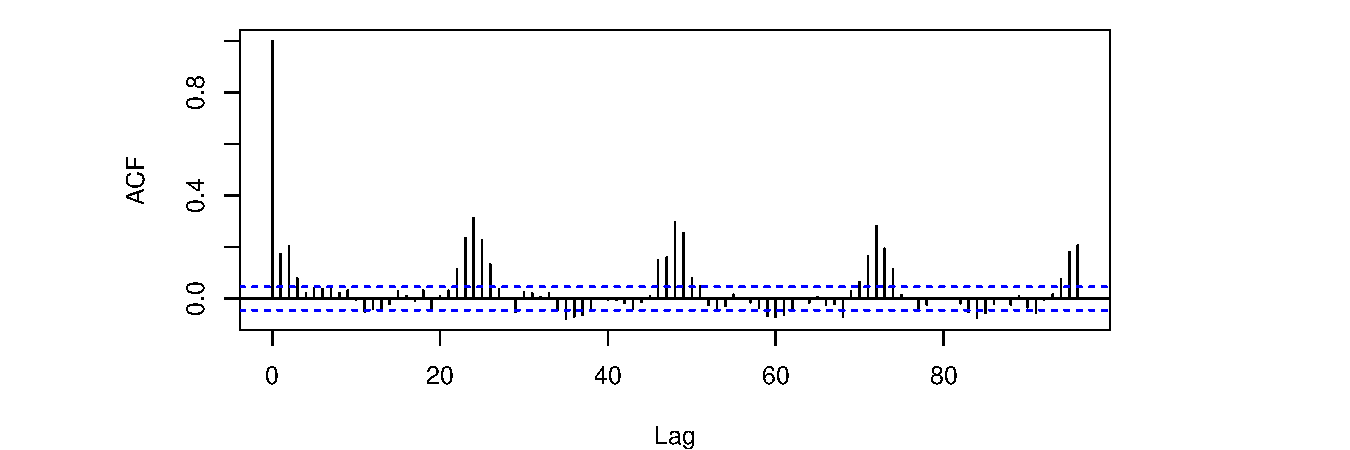
\includegraphics[width=1\linewidth]{tmp/genfig/unnamed-chunk-32-1} 
\end{knitrout}

\noindent The ACF plot suggests that there remains a diurnal pattern to be modelled. It can
be achieved by adding a diurnal curve to the model, e.g.\ with Fourier series
basis functions. This is demonstrated in the vignette \vignette{setup-and-use-model}.

\noindent We may also want to calculate the score as a function of the horizon:
\begin{knitrout}
\definecolor{shadecolor}{rgb}{0.969, 0.969, 0.969}\color{fgcolor}\begin{kframe}
\begin{alltt}
\hlstd{inscore} \hlkwb{<-} \hlstd{D}\hlopt{\$}\hlstd{scoreperiod} \hlopt{&} \hlkwd{complete_cases}\hlstd{(fit}\hlopt{\$}\hlstd{Yhat)}
\hlstd{RMSE} \hlkwb{<-} \hlkwd{score}\hlstd{(}\hlkwd{residuals}\hlstd{(fit),} \hlkwc{scoreperiod} \hlstd{= inscore)}
\hlkwd{plot}\hlstd{(RMSE,} \hlkwc{ylim}\hlstd{=}\hlkwd{c}\hlstd{(}\hlnum{0.75}\hlstd{,}\hlnum{0.88}\hlstd{),} \hlkwc{xlab}\hlstd{=}\hlstr{"Horizon"}\hlstd{)}
\end{alltt}
\end{kframe}

\includegraphics[width=1\linewidth]{tmp/genfig/unnamed-chunk-33-1} 
\end{knitrout}

\noindent The trend is relatively constant, which makes sense since the model is very simple. The offline parameters were optimized for $k=3$
and $k=18$, which can explain why it is not monotonic increasing with the horizon.


%% -- Summary/conclusions/discussion -------------------------------------------

\section{Discussion and conclusion} \label{sec:summary}

%% -- A short discussion on extending functionalities and a conclusion is given in this section.

\subsection{Extending functionality}
The current package is designed to make it easy to implement
new transformation functions and regression schemes, as well as using other
optimizers for tuning parameters.

Implementing a new transformation function is straightforward. The function must receive
either a forecast matrix or a list of forecast matrices and return either after
processing. Furthermore, when used in an online operational setup, where the
transformation is executed whenever new data arrives, it is possible to save state
information inside a transformation function, such that next time the function
is called, the state can be read and used. See the \code{lp()} function for
inspiration when writing a new transformation function.

A new regression scheme, e.g.\ a kernel or quantile regression, can also be
implemented. A fitting function should be implemented in similar way as
\code{lm\_fit()} and \code{rls\_fit()}, such that the first argument is the
parameter vector and it returns a score value, which can be passed to an optimizer.

It is very easy to use other optimizers. The current fitting functions can simply
be passed to any optimizer in \Rprog, which follows the \code{optim()} way of
receiving a function for optimization, see the code in \code{lm\_optim()}.

In future versions of the package, new regression techniques, e.g.\ kernel regression (local
fitting) and quantile regression, might be added. The latter opens up the
possibilities to calculate probabilistic forecasts, see \citep{nielsen2006using}
and \citep{bjerregoard2021introduction}, as
well as carry out normalization and Copula transformations, which can be very
useful for spatio-temporal forecast models, see \citep{tastu2011spatio} or
\citep{lemos2021probabilistic}.


\subsection{Summary and conclusion}

This paper provides an entry point and reference for working with the
\onlineforecast package. The paper covers version 1.0 of the package, which has
been available on CRAN for almost one year at the time of writing.

The main contribution of the package is to make it easy to generate online
multi-step forecasts in a flexible way. The package contains functionalities not
directly available elsewhere, such as:
\begin{itemize}
\item Enabling the use of input variables given as forecasts, e.g.\ NWPs, in an
  easy and flexible way.
\del{\item Modelling of dynamics and non-linearities using transformations including
  tuning the parameters of these transformations.}
\add{\item Optimal tuning of non-linear models for multi-step horizons.}
\item Recursive estimation for tracking time-varying systems computationally
  efficient for multiple horizons.
\end{itemize}
\del{Furthermore, actual online operation with computationally effective
updating is uncomplicated -- so the package is well suited for real-time operational applications.}

The \onlineforecast package has a significant value for anyone who needs to
\del{model}\add{carry out} operational online forecasting, for example, in
energy scheduling, where recursive updated forecasts are needed as input to
optimal decision making and real-time control of systems. It can also be very
useful for companies that need online forecasts for other monitoring and
real-time applications -- specifically, the functionality for model updating with
very little computational costs when new data becomes available, is a unique
feature of the package.



%% -- Optional special unnumbered sections -------------------------------------

\section*{Computational details}
We have tried to make the \onlineforecast package depend on as few other
packages as possible. Only a few additional packages are used in the core
functionalities: \pkg{R6} for the ``usual'' OOP functionalities and \pkg{Rcpp} \citep{eddelbuettel2018}
along with \pkg{RcppArmadillo} \citep{eddelbuettel2014} for easy integration of fast compiled code. For
extending the modelling possibilities the \pkg{splines} and \pkg{pbs} packages
are essential, and for nice caching the \pkg{digest} package was used. We acknowledge the
\pkg{devtools} and \pkg{knitr} \citep{Yihui2015}, \pkg{rmarkdown} \citep{Yihui2018},
\pkg{R.rsp}, \pkg{testthat} \citep{Wickham2011}
packages, which are indispensable for developing a package. We acknowledge
the \Rprog community and the amazing work behind \Rprog done by many people over the
years!

The results in this paper were obtained using \Rprog~4.3.1. \Rprog itself and all packages used are available from the
Comprehensive \Rprog Archive Network (CRAN) at \url{https://CRAN.R-project.org/}.


\section*{Acknowledgments}

The software has been developed with funding from multiple projects:
\add{PTXHeatUtilisation (Energy Cluster Denmark)}, Flexible
Energy Denmark, Heat 4.0 and Decision support tools for smart home energy
management systems (Innovation Fund Denmark, No. 9045-00017B, 8090-00046B and
8053-00156B), TOP-UP (Innovation Fund Denmark and ERA-NET, No. 9045-00017B),
Digital-twin, IEA Annex 71 and 83 Danish participation (EUDP, No. 64019-0570,
64017-05139 and 64020-1007), and finally SCA+ (EU Interreg, No. 20293290).


\bibliography{onlineforecast}



\newpage

\begin{appendix}


\section{Forecast model notation}\label{sec:forec-model-notat}
In this section it is shown how to write \onlineforecast models in mathematical
notation. Both in a full description and how to write a shorter summarized
description. Note, that when variables are noted in bold font it indicates that
they are multi-variate.

A model can be described in full detail as presented in the following.

The transformation stage
\begin{alignat}{2}\label{eq:model-full-trans}
  \text{Intercept:}\quad& \mu_{t+k|t} &\,=\,& 1 \\[1ex]
  \text{Periodic:}\quad& \mB{x}\ns{per}{t+k|t} &\,=\,&  f\n{fs}(t;n\n{har}) \\[1ex]
  \text{Part 1:}\quad& x\ns{1}{t+k|t} &\,=\,& H(B;a) u\ns{1}{t+k|t} \\[1ex]
  \text{Part 2:}\quad& \mB{x}\ns{23}{t+k|t} &\,=\,&
  f\n{bs}(u\ns{2}{t+k|t};n\n{deg}) u\ns{3}{t+k|t} \\[1ex]
  \text{Part 3:}\quad& x\ns{4}{t+k|t} &\,=\,& u\ns{4}{t}
\end{alignat}
and the regression stage
\begin{align}\label{eq:model-full-reg}
  Y_{t+k|t} = \beta_{0,k} \mu_{t+k|t} + \mB{\beta}^T_{1,k}
  \mB{x}\ns{per}{t+k|t} + \beta_{2,k} x\ns{1}{t+k|t} + \mB{\beta}^T_{3,k}
  \mB{x}\ns{23}{t+k|t} + \beta_{4,k} x\ns{4}{t+k|t} + \varepsilon_{t+k|t}
\end{align}

Thus the model inputs are:
\begin{itemize}
\item $t$ is simply the time value.
\item $u\ns{1}{t+k|t}$ some forecast input (e.g.\ NWP variable).
\item $u\ns{2}{t+k|t}$ some forecast input (e.g.\ could be a deterministic
  value, e.g.\ time of day which is always know (the $|t$ could be omitted)).
\item $u\ns{3}{t+k|t}$ some forecast input (e.g.\ NWP variable).
\item $u\ns{4}{t}$ some value at time $t$ (e.g.\ an observation variable).
\end{itemize}
The functions which maps the inputs ($u$'s) to the regression inputs ($x$'s)
are:
\begin{itemize}
\item $f\n{fs}(t;n\n{har})$ is a function generating Fourier series of some
  implicit period length.
\item $H(B;a)$ is a low-pass filter.
\item $f\n{bs}(u\ns{2}{t+k|t};n\n{deg})$ is a function generating basis splines.
\end{itemize}
Their parameters are the transformation parameters:
\begin{itemize}
\item $n\n{har}$ is the number of harmonics.
\item $a$ is the low-pass filter coefficient.
\item $n\n{deg}$ is the degrees of freedom of the spline function.
\end{itemize}
which must be set or optimized.

The regression coefficients are
\begin{align}
  \mB{\beta}_k &= \left[\beta_{0,k} ~~ \mB{\beta}^T_{1,k} ~~ \beta_{2,k} ~~
    \mB{\beta}^T_{3,k} ~~ \beta_{4,k}\right]^T\\
  &=\left[ \beta_{0,k} ~~
    \beta_{1,1,k} ~~ \beta_{1,2,k} ~~ \dots ~~ \beta_{1,2n\n{har},k} ~~ 
    \beta_{2,k} ~~
    \beta_{3,1,k} ~~ \beta_{3,2,k} ~~ \dots ~~ \beta_{3,n\n{deg},k} ~~ 
    \beta_{4,k}\right]^T
\end{align}

If the model is fitted with a recursive scheme, thus the coefficients change
over time, it should be indicated by adding a $t$ to the subscript,
e.g.\ $\beta_{0,k,t}$. Furthermore, other parameters can exist, which can enter
an optimization at the transformation stage, e.g.\ the RLS forgetting factor
$\lambda$. The parameters which are optimized in the transformation stage
should be presented together.

\new{Specifying the model in all details can be cumbersome to include in some texts,
so it makes sense to simplify the notation. When using a simpler notation, as
suggested below, it should be stated, what is implicit (e.g.\ the regression
stage). Referencing the present text should be sufficient when using a simpler
notation. Naturally, all inputs, functions, etc.,\ should be described in some
way.

A model can be specified in a simpler way, e.g.\ the model above in one equation
\begin{align}
  Y_{t+k|t} =&~ \beta_{0,k} + \mB{\beta}^T_{1,k}\, f\ns{fs}{k}(t;n\n{har}) +
    \beta_{2,k}\, H_k(B;a) u\ns{1}{t+k|t} + \mB{\beta}^T_{3,k}\, f\ns{bs}{k}(u\ns{2}{t+k};n\n{deg}) u\ns{3}{t+k|t} \nonumber\\
  &+ \beta_{4,k}\, u\ns{4}{t} + \varepsilon_{t+k|t}
\end{align}
or writing the regression stage implicitly by removing the regression
coefficients where it is meaningful 
\begin{align}
  Y_{t+k|t} = \mu_k + f\ns{fs}{k}(t;n\n{har}) + H_k(B;a) u\ns{1}{t+k|t} + f\ns{bs}{k}(u\ns{2}{t+k|t};n\n{deg}) u\ns{3}{t+k|t} + \beta_k u\ns{4}{t} + \varepsilon_{t+k|t}
\end{align}
It is then implicit that the functions are different from the previous stated
functions, since they include the regression coefficients.} Again, if fitted with
a recursive scheme, then it can be indicated by adding a $t$ subscript,
e.g.\ $f\ns{fs}{k,t}(t;n\n{har})$.

To simplify further the $k$ on the functions can be implicit
\begin{align}
  Y_{t+k|t} = \mu + f\n{fs}(t;n\n{har}) + H(B;a) u\ns{1}{t+k|t} +
  f\n{bs}(u\ns{2}{t+k|t};n\n{deg}) u\ns{3}{t+k|t} + \beta u\ns{4}{t} + \varepsilon_{t+k|t}
\end{align}
and similarly the transformation parameters can be implicit
\begin{align}
  Y_{t+k|t} = \mu + f\n{fs}(t) + H(B) u\ns{1}{t+k|t} +
  f\n{bs}(u\ns{2}{t+k|t}) u\ns{3}{t+k|t} + \beta u\ns{4}{t} + \varepsilon_{t+k|t}
\end{align}
Then the functions and their parameters, and the fitting scheme (i.e.\ with
either LS or RLS for each horizon) should be described in some other way.

Finally, the most simplified notation would be to even remove the time indexing
\begin{align}
  Y = \mu + f\n{fs}(t) + H(B) u\n{1} +
  f\n{bs}(u\n{2}) u\n{3} + \beta u\n{4} + \varepsilon
\end{align}
after making clear how all the variables are defined.

%% <<child="appTransformation.Rnw">>=
%% @ 


\section{Regression} \label{app:regression}

In this section the two regression schemes implemented in \onlineforecast are
described. When fitting a model, thus estimating the regression coefficients,
data from a period $t \in (1,2,\dots,n)$ is used and passed on to either: the
\code{lm\_fit()} function which implements the Least Squares (LS) scheme, or the
\code{rls\_fit()} function, which implements the Recursive Least Squares (RLS) scheme.

One important difference between the two implementations is that in the LS the
coefficients are estimated using data from the entire period, thus they are
constant during the period and the calculated predictions are
``in-sample''. This is opposed to the RLS, where the coefficients are updated
through the period using only past data at each time $t$. In that case the
coefficients vary over time and the calculated predictions are
``out-of-sample''.

This difference is explained in the following and indicated by subscripting the
coefficient vector with $t$ only for the RLS.


\subsection{Least squares}

The regression coefficients for the $k$'th horizon is set in the vector
\begin{align}
  \mB{\beta}_{k} =\left[ \beta_{0,k} ~~
    \beta_{1,k} ~~ \dots ~~ \beta_{p,k} \right]^T
\end{align}
Note, that $t$ is not included in the subscript. 

The input data for the $k$ horizon is the design matrix
\begingroup
% padding
\setlength\arraycolsep{5pt} % space between columns
\renewcommand*{\arraystretch}{2} % space between rows
\begin{align}\label{eq:ls-designmatrix}
  \mB{X}_{k,t} = 
  \begin{bmatrix}
      %%
      x\s{0}{1+k|1} & x\s{1}{1+k|1} & \ldots &
      x\s{p}{1+k|1} \\    
      x\s{0}{2+k|2} & x\s{1}{2+k|2} & \ldots &
      x\s{p}{2+k|2} \\    
      \vdots & \vdots & & \vdots\\
      %%
      x\s{0}{n-1|n-1-k} & x\s{1}{n-1|n-1-k}  &
      \ldots & x\s{p}{n-1|n-1-k}\\
      %%
      x\s{0}{n|n-k} & x\s{1}{n|n-k} & \ldots & x\s{p}{n|n-k}\\
      %%
  \end{bmatrix}
\end{align}
\endgroup

The output observations are in the vector
\begin{align}
  \mB{y}_{k,n} =\left[ y_{1+k} ~~
    y_{2+k} ~~ \dots ~~ y_{n-1} ~~ y_{n}\right]^T
\end{align}

%% The regression model can be written
%% \begin{align}
%%   \mB{y}_{k,n} = \mB{X}_{k,n} \mB{\beta}_{k}
%% \end{align}
The LS estimates of the coefficients are
\begin{align}
  \hat{\mB{\beta}}_{k} = (\mB{X}_{k,n}\mB{X}_{k,n})^{-1} \mB{X}_{k,n}\mB{y}_{k,n}
\end{align}

The predictions are ``in-sample'' and calculated by
\begin{align}
  \hat{\mB{y}}_{k,n} = \mB{X}_{k,n} \hat{\mB{\beta}}_{k}
\end{align}
and returned when fitting a model with \code{lm\_fit()}.

The estimated coefficients may now be used for ``out-of-sample'' prediction (for
$t\n{new} \geq n$), with the input
\begin{align}
  \mB{x}_{t\n{new}+k|t\n{new}} = \left[ x\s{0}{t\n{new}+k|t\n{new}} ~~ x\s{1}{t\n{new}+k|t\n{new}} ~~ \dots ~~
    x\s{p}{t\n{new}+k|t\n{new}} \right]^T
\end{align}
by
\begin{align}
  \hat{y}_{t\n{new}+k|t\n{new}} = \mB{x}_{t\n{new}+k|t\n{new}} \hat{\mB{\beta}}_{k} 
\end{align}
This can be done by providing new data to the \code{lm\_predict()} function.



\subsection{Recursive least squares}

In the RLS scheme the coefficients are recursively updated through the
period. Time $t$ steps from 1 to $n$ and in each step the ``newly'' obtained
data at $t$ is used for calculating updated coefficients. The coefficient vector
has the same structure as for LS
\begin{align}
  \mB{\beta}_{k,t} =\left[ \beta_{0,k,t} ~~ \beta_{1,k,t} ~~ \dots ~~ \beta_{p,k,t} \right]^T
\end{align}
The only difference is that we now subscript with $t$ because it varies over
time.

Only the most recent input data at $t$ (the row at $t$ from the LS design
matrix in Equation \eqref{eq:ls-designmatrix}) is used in each update
\begin{align}
  \mB{x}_{k,t} = \left[ x\s{0}{t|t-k} ~~ x\s{1}{t|t-k} ~~ \dots ~~
    x\s{p}{t|t-k} \right]^T
\end{align}  
and similarly the most recent output observation $y_{t}$. At each time $t$ the coefficients are updated by
\begin{align}
  \mB{R}_{k,t} &= \lambda \mB{R}_{k,t-1} + \mB{x}_{k,t} \mB{x}^T_{k,t}\\
  \hat{\mB{\beta}}_{k,t} &= \hat{\mB{\beta}}_{k,t-1} + \mB{R}^{-1}_{k,t}
  \mB{x}_{k,t} (y_t - \mB{x}^T_{k,t} \hat{\mB{\beta}}_{k,t-1})
\end{align}

Hence, when applying RLS for data from the period $t \in (1,2,\dots,n)$ the
RLS provides a new value of the coefficients for each time $t$ (opposed to LS).

The predictions are calculated recursively as well by using the updated
coefficients at each time $t$. Given the inputs
\begin{align}
  \mB{x}_{t+k|t} = \left[ x\s{0}{t+k|t} ~~ x\s{1}{t+k|t} ~~ \dots ~~
    x\s{p}{t+k|t} \right]^T
\end{align}
the prediction is
\begin{align}
  \hat{y}_{t+k|t} = \mB{x}_{t+k|t} \hat{\mB{\beta}}_{k,t}
\end{align}
Only past data has been used when calculating the predictions through the
period, hence they are ``out-of-sample'' predictions (these predictions are returned by \code{rls\_fit()}).

The initial value of $R$ is set simply set to a zero matrix with diagonal
$1/10000$ and $\beta$ set to a zero vector.

An alternative updating scheme, which is actually the implemented scheme (gives
the same results as the scheme above), is the Kalman gain scheme
\citep{sayed1994state}, where matrix inversion is avoided
\begin{align}
  \mB{K}_{k,t} &= \frac{\mB{P}_{k,t-1} \mB{x}_{k,t}}{ \lambda + \mB{x}^T_{k,t}
    \mB{P}_{k,t-1} \mB{x}_{k,t}}\\
  \hat{\mB{\beta}}_{k,t} &= \hat{\mB{\beta}}_{k,t-1} + \mB{K}_{k,t} (y_t -
  \mB{x}^T_{k,t} \hat{\mB{\beta}}_{k,t-1})\\
  \mB{P}_{k,t} &= \frac{1}{\lambda} \left( \mB{P}_{k,t-1} - \mB{K}_{k,t}
  \mB{x}^T_{k,t} \mB{P}_{k,t-1} \right)
\end{align}
This actually opens up the possibilities for self-tuned variable forgetting
\citep{shah1991recursive}.


\end{appendix}


\address{
Peder Bacher\\
Dynamical Systems, Department of Applied Mathematics and Computer Science, Technical University of Denmark\\
Asmussens Allé, Building 303B\\
2800 Kgs. Lyngby, Denmark\\
E-mail: \email{pbac@dtu.dk}\\
URL: \url{https://www.compute.dtu.dk/english/research/research-sections/dynsys/}
}

\address{
Hjörleifur G. Bergsteinsson\\
Dynamical Systems, Department of Applied Mathematics and Computer Science, Technical University of Denmark\\
Asmussens Allé, Building 303B\\
2800 Kgs. Lyngby, Denmark\\
E-mail: \email{hgbe@dtu.dk}\\
URL: \url{https://www.compute.dtu.dk/english/research/research-sections/dynsys/}
}

\address{
Linde Frölke\\
Dynamical Systems, Department of Applied Mathematics and Computer Science, Technical University of Denmark\\
Asmussens Allé, Building 303B\\
2800 Kgs. Lyngby, Denmark\\
E-mail: \email{hgbe@dtu.dk}\\
URL: \url{https://www.compute.dtu.dk/english/research/research-sections/dynsys/}
}

\address{
Mikkel L. Sørensen\\
Dynamical Systems, Department of Applied Mathematics and Computer Science, Technical University of Denmark\\
Asmussens Allé, Building 303B\\
2800 Kgs. Lyngby, Denmark\\
E-mail: \email{mliso@dtu.dk}\\
URL: \url{https://www.compute.dtu.dk/english/research/research-sections/dynsys/}
}

\address{
Julian Lemos-Vinasco\\
Dynamical Systems, Department of Applied Mathematics and Computer Science, Technical University of Denmark\\
Asmussens Allé, Building 303B\\
2800 Kgs. Lyngby, Denmark\\
E-mail: \email{jlvi@dtu.dk}\\
URL: \url{https://www.compute.dtu.dk/english/research/research-sections/dynsys/}
}

\address{
Jon Liisberg\\
Dynamical Systems, Department of Applied Mathematics and Computer Science, Technical University of Denmark\\
Asmussens Allé, Building 303B\\
2800 Kgs. Lyngby, Denmark\\
E-mail: \email{jlvi@dtu.dk}\\
URL: \url{https://www.compute.dtu.dk/english/research/research-sections/dynsys/}
}

\address{
Jan Kloppenborg Møller\\
Dynamical Systems, Department of Applied Mathematics and Computer Science, Technical University of Denmark\\
Asmussens Allé, Building 303B\\
2800 Kgs. Lyngby, Denmark\\
E-mail: \email{jkmo@dtu.dk}\\
URL: \url{https://www.compute.dtu.dk/english/research/research-sections/dynsys/}
}

\address{
Henrik Aalborg Nielsen \\
ENFOR A/S\\
Røjelskær 11, 3. \\
2840 Holte, Denmark\\
E-mail: \email{han@enfor.dk}\\
URL: \url{https://www.enfor.dk}
}

\address{
Henrik Madsen\\
Dynamical Systems, Department of Applied Mathematics and Computer Science, Technical University of Denmark\\
Asmussens Allé, Building 303B\\
2800 Kgs. Lyngby, Denmark\\
E-mail: \email{hmad@dtu.dk}\\
URL: \url{https://www.compute.dtu.dk/english/research/research-sections/dynsys/}
}

\end{article}

\end{document}
